

\section*{Binomial Example }

Suppose a die is tossed 5 times. What is the probability of getting exactly 2 fours?

\subsection*{Solution:}

This is a binomial experiment in which \begin{itemize}\item a success is defined as an outcome of `4'. \item the number of trials is equal to $n=5$, \item the number of successes is equal to $k=2$,\item the number of failures is equal to 3, \item  the probability of success on a single trial is 1/6, \item  the probability of failure on a single trial is 5/6.\end{itemize}

\smallskip

Therefore, the probability of getting exactly 2 fours is:

\[P(X=2) = ^5C_2 \times (1/6)^2 \times (5/6)^3 = 0.161\]

Remark: $^5C_2 = 10$\\
\bigskip

\begin{center}
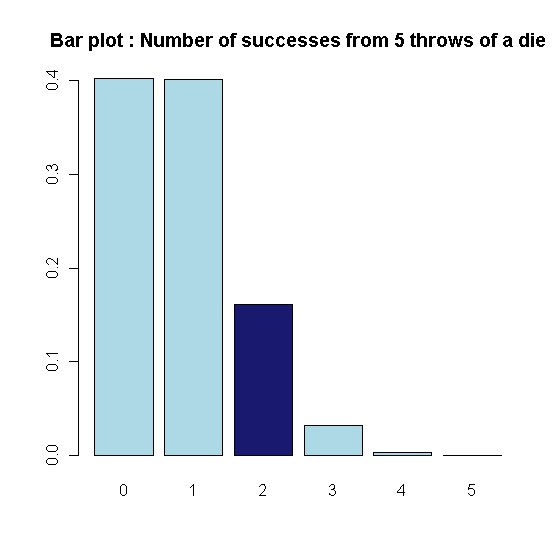
\includegraphics[scale=0.40]{images/3Bbarplot4}
\end{center}


\subsection*{Remark}  The sum of the probabilities of each of the possible outcomes (i.e. no fours, one four etc) is equal to one.
\[P(X=0) + P(X = 1) + \ldots + P(X=5) = 1 \]


\subsection*{Binomial Example: At least two successes}

\begin{center}
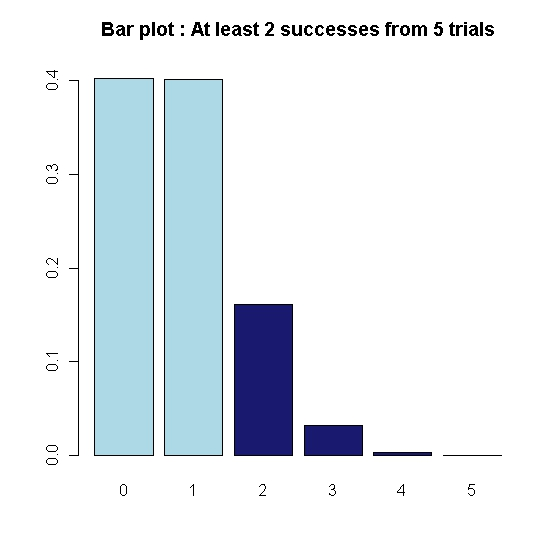
\includegraphics[scale=0.40]{images/3Bbarplot5}
\end{center}


\begin{itemize}
\item Suppose we were asked to find the probability of \textbf{\emph{at least}} 2 fours.
\item Can you suggest the most efficient way of computing this?
\item Suggestion: Compute $P(X=0)$ and $P(X = 1)$.
\item Together these probabilities are the complement probability of what we require.
\item $P(X \geq 2) = 1 - ( P(X=0) + P(X = 1))$.
\end{itemize}
\newpage


%--------------------------------------------------------------------------------------%
\frame{
\frametitle{ Binomial Example 1 }
(Revision from Last Class)\\
Suppose a die is tossed 5 times. What is the probability of getting exactly 2 fours?

\textbf{Solution:} This is a binomial experiment in which the number of trials is equal to 5, the number of successes is equal to 2, and the probability of success on a single trial is 1/6 or about 0.167. 
\\
\bigskip
Therefore, the binomial probability is:

\[P(X=2) = ^5C_2 \times (1/6)^2 \times (5/6)^3 = 0.161\]
}

%--------------------------------------------------------------------------------------%
\frame{
\frametitle{ Binomial Example 2 }
Suppose there is a container that contains 6 items.  The probability that any one of these items is defective is 0.3. Suppose all six items are inspected. 
\begin{itemize}
\item What is the probability of 3 defective components?
\item What is the probability of 4 defective components?
\end{itemize}

\[ P(3\text{ defects}) = f(3) = P(X = 3) = {6\choose 3}0.3^3 (1-0.3)^{6-3} = 0.1852 \]
\[ P(4\text{ defects}) = f(4) = P(X = 4) = {6\choose 4}0.3^4 (1-0.3)^{6-4} = 0.0595 \]
}
